\chapter{Models and Associated Probes For Proton Spin Structure}
\label{ch:modeling_proton_spin}

With the advances made over the last half-century, we have come very close to
obtaining a complete model describing the world around us.  Rapid progress has
been made in the last 40 years in the understanding of the structure of the
nucleon. Protons and neutrons make up the majority of the mass in the visible
universe--therefore understanding their nature completely is of fundamental
importance to physics.

In the previous chapter, we discussed in the history behind studying the
structure of matter, leading up to a brief discussion of the contemporary
experiments in proton spin structure. Glaringly, I neglected to discuss the
Relativistic Heavy Ion Collider (RHIC) and the Pioneering High Energy Nuclear
Interaction eXperiment (PHENIX), since I wanted to put the program into a firm
theoretical context in this chapter.

This thesis will discuss the experimental efforts of PHENIX to do something no
other experiment has done--utilize the production of $W$ Bosons as a direct probe
of proton spin. Before we discuss the specifics of this measurement, lets first
put proton spin into a larger context.

\section{Modeling the Proton Structure}

One frequent theme in using particle accelerators to study any kind of nuclear
structure is that we do not ever get to directly look at the innards of a
proton, due to the phenomena of color confinement.

This means that often, we must deal with the process of how partons (quarks,
gluons) fragment and decay after a proton proton collision. Additionally, we
must deal with and account for the scale-variance of the fundamental forces. 

The scale variance of the fundamental forces has large implications for the
strong nuclear force, generally represented by the coupling constant,
$\alpha_S$. This constant scales with distance, and becomes highly
non-perturbative at short distances. Writing models in high energy physics can
be created to describe perturbative processes or non-perturbative models.  In
perturbative models, the general strategy is to write down a Hamiltonian or
Lagrangian to describe a system, and then obtain predictions from the model by
expanding in terms of a `small' parameter. Then, predictions from the leading
order, NLO, NNLO or NNNLO are made and verified with data. Non perturbative
models often cannot write down the final solution to some differential equation
which is thought to describe a solution--so instead, experiments are designed
to constrain these models with data. The models can then make more predictions
which can again be verified with experiments. 

The internal degrees of freedom of the proton, and the small scales involved
make models for the proton fall generally into non-perturbative regimes. We find
that the very structure and distribution of partons and gluons in the nucleus is
a scale-dependent phenomena, that is to say, if we take measurements at a lower
energy, we get a different distribution of partons and gluons than if we measure
at higher energy. This scale dependence requires many measurements to be taken
which probe different scales in order to properly constrain models for proton
structure. 

In order to properly model the non-perturbative structure of the proton, we use
a Factorization Theorem, which provides us a way to mathematically separate an
probing interactions (such as electron-hadron scattering in DIS) into
perturbative and non-perturbative parts (example,
Figure~\ref{fig:disschematic}). The non-perturbative aspect in the figure (the
X) is often the portion which is experimentally constrained.

Because modern models for proton structure treat the particle as a largely
non-perturbative object we create distribution functions which are
experimentally measured (or constrained) to handle predictions of the proton's
properties which arise from non-perturbative processes. One such property is the
spin of the proton, which must arise in some way from the interactions of the
quarks and gluons which swirl about inside of the proton.

As a note here, for this work on theoretical background of deep inelastic
scattering in the first portion of this chapter, I reference Dr. Ciprean Gal's
clear and coherent introduction to the subject, published in
2014~\cite{Gal2014b}, in his thesis describing the complimentary analysis done
at PHENIX at central rapidities. Later on, I will more heavily rely on Dr.
Oide's work published in his respective thesis.  Thanks guys!

\subsection{Structure Functions}
\label{sec:structure_functions}

Given that the proton itself has so far been shown to be a non-perturbative
object, we need a means to model the structure of the interaction when two
protons collide, and generate particles.  Generally, we can calculate a
structure function associated with each hadronic process. The variables we
define to describe the kinematics of deep inelastic scattering are (see
Figure~\ref{fig:disschematic}):

\begin{gather}
  P \label{eq:P}\\
  Q^2 \equiv -q^2 \label{eq:big_q_sq}\\
    x \equiv { Q^2 \over {2P\cdot q} } \label{eq:x}
\end{gather}

$P$ is the total hadron momentum (in our case, the proton's momentum), $Q^2$ is
the energy exchange between the proton and probe lepton, and $x$ is the fraction
of the total proton's momentum carried by the quark scattering with the lepton.
$q$, in Equation~\ref{eq:x} is four-momentum transferred from the lepton to the
quark. 

We can then write down structure functions in terms of these variables. We have:

\begin{gather}
  F_1(x,Q^2) = {1 \over 2}\sum_f e_f^2 \left(q_f(x)+\bar{q}(x)\right)
  \label{eq:f1} \\
  F_2(x,Q^2) = 2xF_1(x,Q^2)\label{eq:f2}
\end{gather}

The subscript, $f$ refers to the quark flavors represented in the structure
functions, with $e_f$ referring to the charge of each quark being summed over
(i.e. ${\pm}{1\over3}$ or ${\pm}{2\over3}$). $q(x)$ refers to the parton
distribution function associated with each quark flavor. 

An integration over the momentum fraction, $x$ of Equation~\ref{eq:f2} and the
gluon structure function $g(x)$ yields the familiar `valence quark' structure of
the proton, i.e. two up-quarks and one down quark, with remaining quark flavors
$q_h$ summing to zero:

\begin{gather}
	\int_0^1 F_2(x,Q^2) + g(x) dx 
	= \int_0^1 
	\left(
		x\sum_f e_f^2 \left(q_f(x)+\bar{q}(x)\right) 
	\right) 
	+ g(x) dx \label{eq:f2_int_1} \\
	\int_0^1 \left(u(x)+\bar{u}(x) dx \right) dx = 2  \label{eq:up_quark_valence} \\
	\int_0^1 \left(d(x)+\bar{d}(x) dx \right) dx = 1  \label{eq:down_quark_valence} \\
	\int_0^1 \left(q_h(x)+\bar{q}_h(x) dx \right) dx = 0 \label{eq:other_quark_valence}
\end{gather}

The rest of the world data on $F_2(x,Q^2)$ is summarized in
Figure~\ref{fig:f2_world_data}

\begin{figure}[ht]
  \centering
  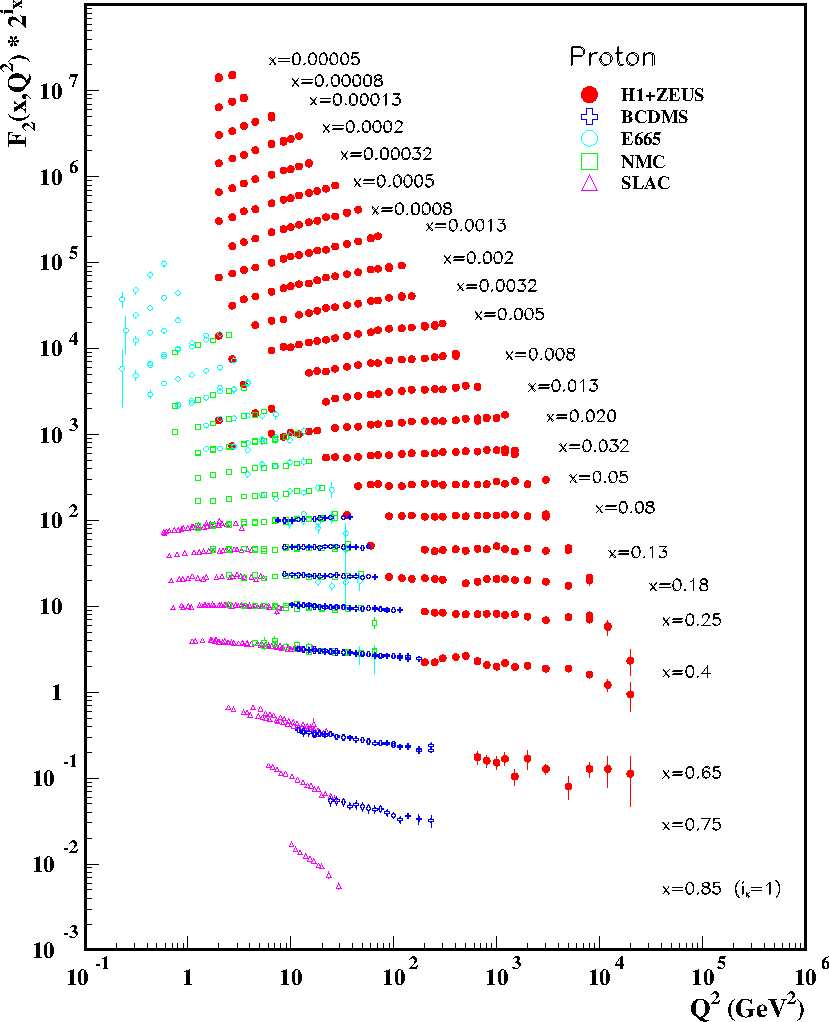
\includegraphics[width=\linewidth]{./figures/F2_structure_function.pdf}
  \caption{
		Here, we see "the proton structure function, $F_2^p$ measured in
		electromagnetic scattering experiments of electrons and positrons on
		protons" from experiments including H1+Zeus, BCDMS, E665, NMC and
		SLAC~\cite{ReviewEidelman2012}
  }
  \label{fig:f2_world_data}
\end{figure}

\clearpage
\section{Parton Distribution Functions}
\label{sec:parton_distribution_functions}

From this dataset, we can extract Parton Distribution Functions for any
combination of $x$ and $Q^2$. Under this particular framework, we can use the
DGLAP evolution equations to evolve PDFs observed at one $Q^2$ to some other
$Q^2$~\cite{Altarelli2009}.

With QCD evolution, one can additionally undertake a global analysis, which
effectively puts a constraint on Parton Distribution functions using `evolved
projections' of $x$ and $Q^2$ into the kinematic range of the experimental
probes~\cite{Gal2014b}. 

The world data on proton structure can by evolved with the DGLAP
equations~\cite{Ellis1974} to generate parton distribution functions
representing the momentum fraction carried by various partons building up the
proton, the summary of this is shown in Figure~\ref{fig:unpolarized_pdf}.

\begin{figure}[ht]
  \centering
  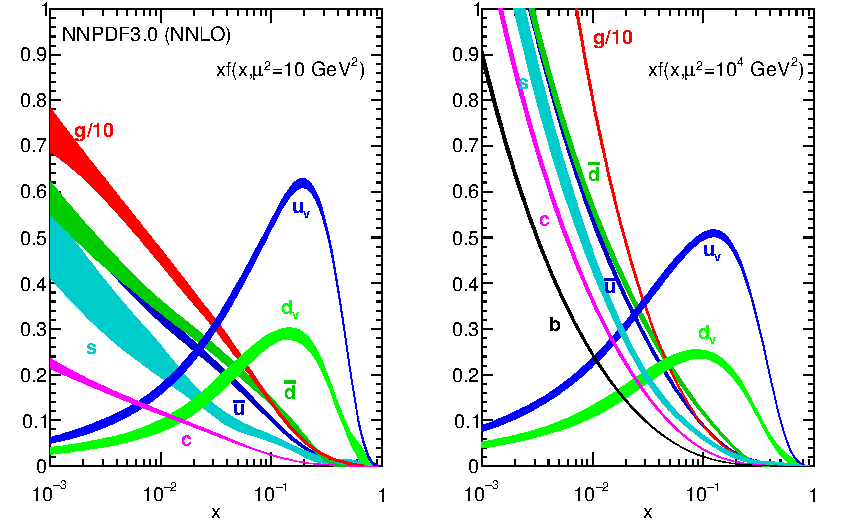
\includegraphics[width=0.7\linewidth]{./figures/unpolarized_pdfs.pdf}
  \caption{
    Here, we see as expected--the PDF for $u$ is about twice as large as $d$
    indicating the valence structure of the proton at high-x ($>0.1$). On the
    left is the NNPDF calculation of PDFs with world data (width is related to
    uncertainty) at 10 GeV, while 10 TeV is shown on the right. Note that at
    low $x$, the proton is dominated by gluons.~\cite{ReviewEidelman2012}.
  } 
  \label{fig:unpolarized_pdf}
\end{figure}

While DIS, and Semi-Inclusive Deep Inelastic Scattering have provided a wealth
of data on the proton's internal structure--we have the advantage at RHIC to
undertake a complimentary analysis, using hadron-hadron collisions, instead of
hadron-lepton collisions. A similar picture to DIS can be drawn of
hadron-hadron interactions to the DIS schematic, as seen in
Figure~\ref{fig:hadron_inelastic_scattering}.

\begin{figure}[ht]
  \centering
	\begin{subfigure}{0.5\textwidth}
		\centering
		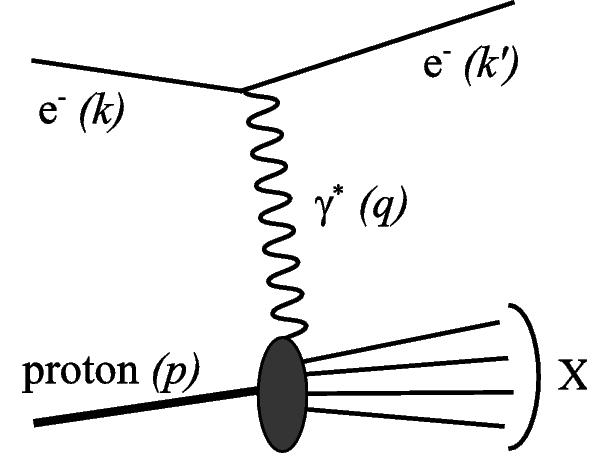
\includegraphics[width=\textwidth]{./figures/deep_inelastic_basic.png}
    \caption{Leptonic Deep Inelastic Scattering}
		\label{fig:dis}
	\end{subfigure}%
	\begin{subfigure}{0.5\textwidth}
		\centering
		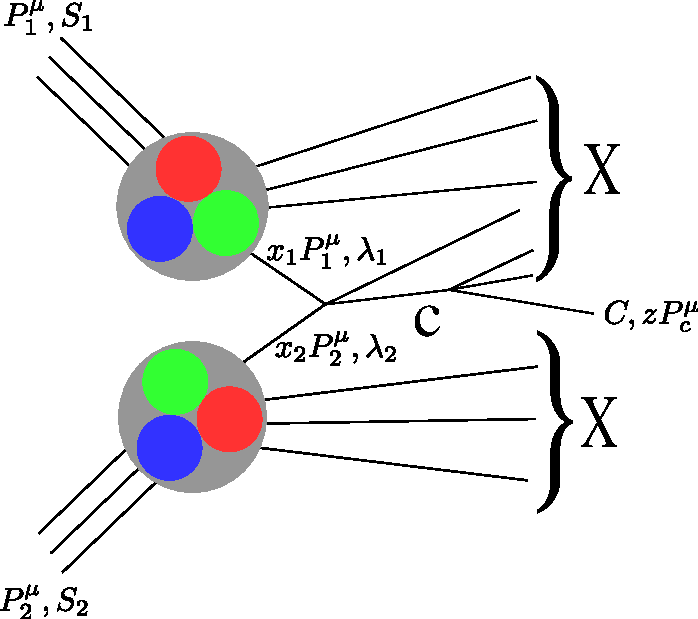
\includegraphics[width=\textwidth]{./figures/hadron_inlastic_scattering.pdf}
    \caption{Hadronic Inelastic Scattering}
    \label{fig:his}
	\end{subfigure}
  \caption{
    Deep Inelastic Scattering Process (left) alongside Hadron-Hadron inelastic
    scattering (right). In hadron inelastic scattering, one may try to select
    initial state with scattering between arbitrary partons in order to probe
    various proton structures.
  }
  \label{fig:hadron_inelastic_scattering}
\end{figure}

Hadron-Hadron scattering can be a useful means to determine PDFs experimentally,
but often intermediate states are not known and it is difficult to isolate a
single PDF. Hadron-hadron scattering experiments are an excellent way to
constrain gluon PDFs.

\subsection{Polarized Parton Distribution Functions}
\label{sec:polarized_parton_distribution_functions}

Polarized parton distributions are measured with the same methods discussed
above--except the beam and target in the scattering formalism are
spin-polarized. We can similarly write down the structure functions for
polarized protons, in the same manner as $F_1$ and $F_2$:

\begin{equation}
  g_1 = {1 \over 2}\sum_q e_q^2(q^+(x)-q^-(x)) 
  = {1 \over 2} \sum_q e^2_q\Delta q(x)
  \label{eq:g1}
\end{equation}

Here, $e_q$ is the charge of the quark-flavor (i.e., $1/3e$, $2/3e$), with the
sum taken over all quark/anti-quark flavors. The $q$ terms refer to the number
density of each particularly quark flavor associated with the ``+'' or ``-'' quark
spin orientation (relative to the struck hadron), such that ``+'' refers to a
parallel spin and ``-'' refers to an anti-parallel spin. $g_1$ describes the
longitudinal spin polarization of the nucleus, while $g_2$ describes the
transverse spin polarization of the nucleus. A knowledge of both longitudinal
and transverse spin structure is necessary for a complete understanding of the
three-dimensional structure of the proton. This thesis presents my analysis of
the longitudinal spin structure, so I will leave a further discussion of $g_2$
in the capable hands of my colleagues.  

The experimental tool for measurement of the spin structure of the proton is the
`spin asymmetry'. The spin asymmetry is defined in two ways--one, through
cross-sections, which crucially, may be additionally defined in terms of the
structure functions. For any value of $x$ and $Q^2$, we may write down the
asymmetry:

\begin{align}
  A(x,Q^2) &= {{\sigma^+-\sigma^-}\over{\sigma^++\sigma^-}} \label{eq:al_simple} \\
           &\equiv {{g_1(x,Q^2)}\over{F_1(x,Q^2)}} \label{eq:al_structure}
\end{align}

With our knowledge of $F_1$ from fits to the world's data, we can use the
asymmetry to measure $g_1$ directly. With the discovery that the proton's spin
is not entirely carried by the valence quarks, we can construct additional
spin-dependent parton distribution functions, and design experiments to measure
and constrain them. Thus far, the world's data to do so has been used to
generate predictions of these PDFs summarized in Figures
\ref{fig:polarized_pdfs_1} and \ref{fig:polarized_pdfs_2}.

\begin{figure}[ht]
  \centering
  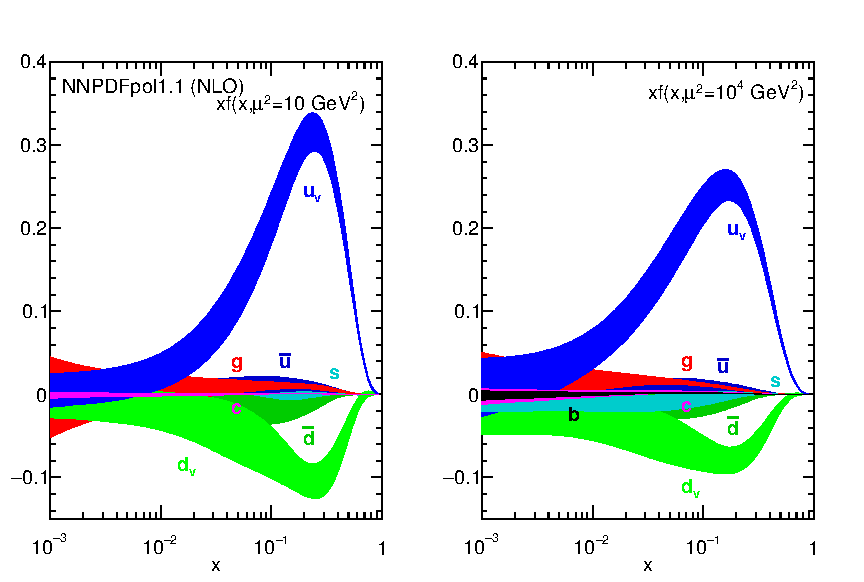
\includegraphics[width=0.7\linewidth]{./figures/polarized_pdfs.pdf}
  \caption{
    World data used to generate fits to predict the parton distribution
    functions of various quark flavors in the proton at 10 GeV (left) and 10
    TeV (right)~\cite{ReviewEidelman2012}
  }
  \label{fig:polarized_pdfs_1}
\end{figure}

\begin{figure}[ht]
  \centering
  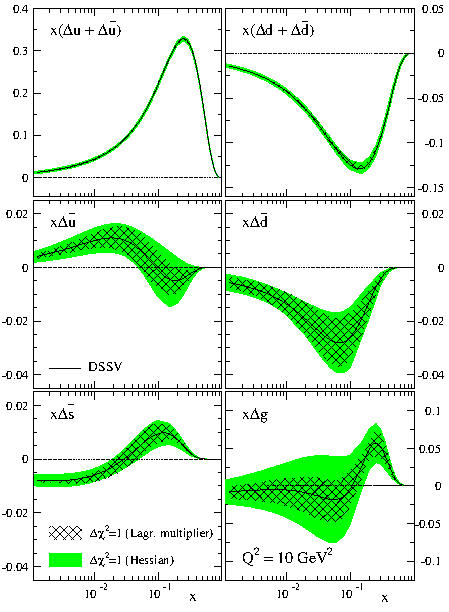
\includegraphics[width=0.8\linewidth]{./figures/polarized_pdfs_dssv.pdf}
  \caption{
    de Florian, Vogelsang, Sassot and Stratmann produced predictions at 10 GeV
    for the PDFs for quarks and anti-quarks and gluons in the proton. The
    uncertainties for the gluon and anti-quark PDFs are quite large, warranting
    experimental investigation~\cite{DeFlorian2009}.
  }
  \label{fig:polarized_pdfs_2}
\end{figure}

\clearpage
\section{Proton Spin Decomposition with the Ellis-Jeffe Sum Rule }

We may write down the spin contribution of the proton as a sum of the various
spin contributions via the polarized parton distribution functions of the
partons inside the proton in various gauges:

{\noindent}Gauge invariant Ellis-Jeffe
\begin{equation}
  \braket{P,{1\over2}|\hat{J_z}|P,{1\over2}}  
 = {1\over2} = {{1\over2}\Delta \Sigma +L_q+J_g}
\label{eq:ellis_jeffe_sum}
\end{equation}

{\noindent}Infinite momentum decomposition:
\begin{equation}
  \braket{P,{1\over2}|\hat{J_z}|P,{1\over2}}  
  = {1\over2} = {{1\over2}\Delta \Sigma +L_q+\Delta g + L_g}
  \label{eq:infmom_ellis_jeffe_sum}
\end{equation}

{\noindent}Quark decomposition:
\begin{equation}
  {\Delta \Sigma} =
  {
    (\Delta u+\Delta \bar{u})
    +(\Delta d + \Delta \bar{d})
    +(\Delta s + \Delta \bar{s})
  }
  \label{eq:quark_spin_decomposition}
\end{equation}

There is a large uncertainty in the contribution of the anti-quarks to the
proton spin \ref{eq:quark_spin_decomposition}, which this thesis will seek to
constrain.

\section{The Spin Asymmetry: An Experimental Probe }

As discussed in the previous sections, the spin asymmetry is an important
experimental probe into the longitudinal spin structure function, $g_1$ from
which we can derive polarized parton distribution functions. At RHIC, we can use
hadron inelastic scattering to construct asymmetries for various final-states to
measure and constrain the parton distribution function. These probes are
summarized in Figure~\ref{fig:spin_probes_masterspin}.

\begin{figure}[ht]
  \centering
  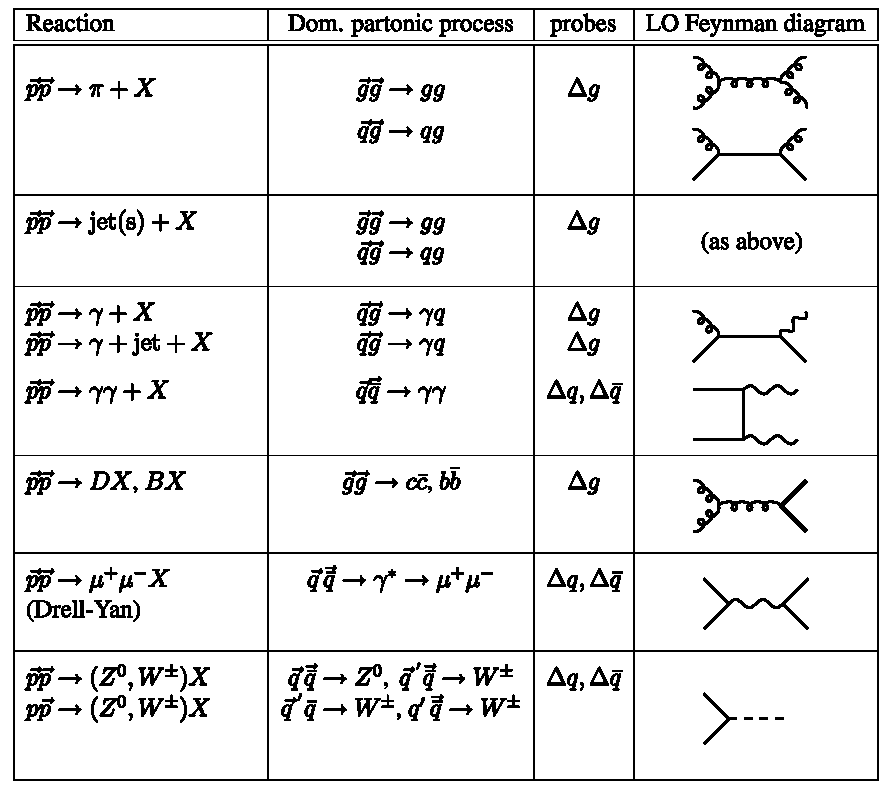
\includegraphics[width=\linewidth]{./figures/spin_probes.pdf}
  \caption{
    A summary of the various probes for longitudinally polarized protons. The
    \textbf{``Reaction''} column summarizes the reaction observed experimentally.
    The \textbf{``Dom. partonic process''} column describes the dominant process
    at the partonic level. The \textbf{``probes''} column shows which proton spin
    structure can be measured with the reaction. Finally, the leading order
    Feynman diagram for the partonic process is drawn. Figure is reproduced
    from: \cite{Aidala2005}.
  }
  \label{fig:spin_probes_masterspin}

\end{figure}

One potential pit-fall of using hadronic initial states in spin measurements is
the issue of fragmentation. It can be difficult to construct a clean probe,
since often, the final measured state can be something like a photon decay from
a $\pi^0$--and these $\pi^0$'s can be produced in a vast array of fragmentation
processes. It can be hard to isolate the parent interaction which produced the
particles of interest. However, the production of $W$ Bosons offers a clean probe
free of fragmentation into the polarization of anti-quark parton distribution
functions. While all weak processes are mediated by the W/Z boson, real $W$ Boson
production from $q+\bar{q}$ interaction produces a clear Jacobean peak at
central rapidities at the 510 GeV $\sqrt{s}$ collision energy of interest, and
additionally can be identified at forward rapidities using statistical methods
discussed later.

\clearpage
\section{W Production}

Though $W$ Bosons obviously can be created in collisions with the right
ingredients and correct energy, the $W$ Bosons that we're interested in at RHIC
are very special. The collision conditions around the protons at colliding at
PHENIX provides just enough energy to create real $W$ Bosons from interaction of
quarks and anti-quarks between two colliding protons. The energy is not
sufficiently high enough to produce real $W$ Bosons from other processes in
amounts which would significantly dilute the primary source.

The standard model tells us that W production occurs through a pure vector-axial
interaction, this implies that the helicity of the parents particles--in
particular $u+\bar{d}\rightarrow W^+$ and $\bar{u}+d\rightarrow W^-$ have fixed
helicities, due to the relativistic final state neutrino (which is not measured,
of course). To visualize the leading order of W production, with regards to the
quark-sea element being probed, the leading order diagrams for the interaction
are shown in Figure~\ref{fig:w_probe_leading_order}~\cite{Aidala2005}

Since $\Delta q$, the polarized parton distribution function can be split into
contributions from valence quarks, and also sea quarks, understanding $\Delta
\bar{q}$ is an important step towards understanding $\Delta q$ better to better
understand the total proton spin.

\begin{figure}[ht]
  \centering
  \begin{subfigure}[b]{\textwidth}
    \centering
    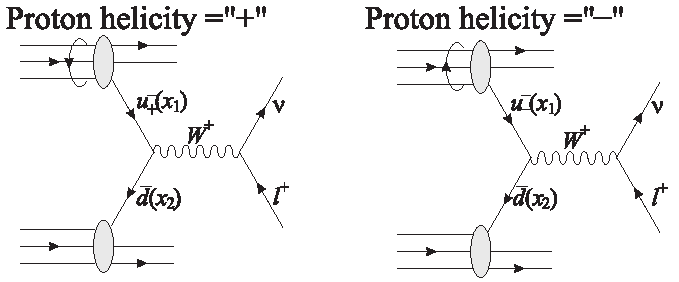
\includegraphics[width=0.8\linewidth]{./figures/w_plus_u_probe.pdf}
    \caption{
      Probe for $\Delta u$ at lowest order.
    }
    \label{fig:u_probe}
  \end{subfigure}
  \begin{subfigure}[t]{\textwidth}
    \centering
    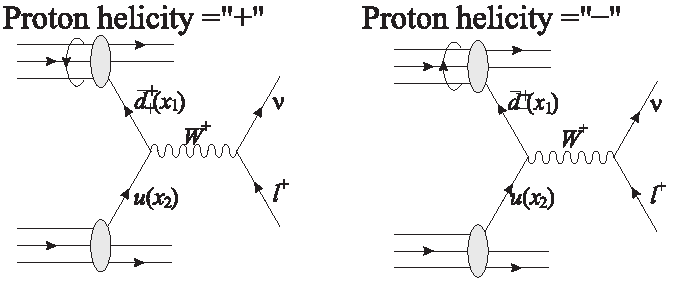
\includegraphics[width=0.8\linewidth]{./figures/w_plus_dbar_probe.pdf}
    \caption{
      Probe for $\Delta\bar{d}$ at lowest order
    }
    \label{fig:dbar_probe}
  \end{subfigure}
  \caption{
    Real $W^+$ production as produced at PHENIX. The helicity of the initial
    state fixes the helicity of the partonic participants due to the
    relativistic final state of the neutrino + the handedness of the $W$ Boson.
    $x_1$ and $x_2$ are the momentum fractions of the quarks participating from
    the participant partons~\cite{Aidala2005}. 
  }
  \label{fig:w_probe_leading_order}
\end{figure}

Though both protons in the collision are polarized, the polarization of one
participant proton can be effectively ignored by summing over all polarization
states for one of the two protons. With this assumption, we may construct a
single spin asymmetry for colliding protons by counting difference in the number
of positively and negatively polarized W's produced in collisions, scaled by the
total production:

\begin{equation}
  {{A_L}^W} =
  {{{1}\over{P}}\times{{N_{-}(W)-N_{+}(W)}\over{{N_{-}(W)+N_{+}(W)}}} }
  \label{eq:w_production_asymmetry}
\end{equation}

This is a relatively easy experimental probe to measure (assuming that we can
accurately count events which produced a W, which naturally, is nearly
impossible, as we will see in Section~\ref{sec:sbr}).

As we saw earlier, in
Section~\ref{sec:polarized_parton_distribution_functions}, we can write an
asymmetry in terms of the scattering cross section for the process responsible
for particle yields. These cross-sections were shown to be written in terms of
polarized parton distribution functions, thus, we cut to the chase to write
down the full expression of the theoretical asymmetries for this process in
terms of those parton distribution functions.

The following equations all contain an implied integration over $x_1$ and $x_2$.

For $W^+$ and $u$:
\begin{equation}
  {A_L^{W^+}} = 
  {
    {u_-^-(x_1)\bar{d}(x_2)-u_+^-(x_1)\bar{d}(x_2)}
    \over
    {u_-^-(x_1)\bar{d}(x_2)-u_+^-(x_1)\bar{d}(x_2)}
  }  
  \label{eq:al_u_full}
\end{equation}

For $W^+$ and $\bar{d}$
\begin{equation}
  {A_L^{W^+}} = 
  {
    {\bar{d}_-^+(x_1)u(x_2)-\bar{d}_+^+(x_1)u(x_2)}
    \over
    {\bar{d}_-^+(x_1)u(x_2)+\bar{d}_+^+(x_1)u(x_2)}
  }  
  \label{eq:al_dbar_full}
\end{equation}

Observationally, we see a superposition of \ref{eq:al_u_full} and
\ref{eq:al_dbar_full}, which is expressed in
Equation~\ref{eq:al_superposition_pos}:

\begin{equation}
  {A_L^{W^+}} = 
  {
    {
      \Delta u(x_1)\bar{d}(x_2)-\Delta \bar{d}(x_1)u(x_2)
    }
    \over
    {
      u(x_1)\bar d(x_2)+\bar(d)(x_1)u(x_2)
    }
  }
  \label{eq:al_superposition_pos}
\end{equation}

For the case of $W^-$, we observe $\bar{d}$ and $u$:
For $W^-$ and $d$:
\begin{equation}
  {A_L^{W^+}} = 
  {
    {d_-^-(x_1)\bar{u}(x_2)-d_+^-(x_1)\bar{u}(x_2)}
    \over
    {d_-^-(x_1)\bar{u}(x_2)-d_+^-(x_1)\bar{u}(x_2)}
  }  
  \label{eq:al_d_full}
\end{equation}

For $W^-$ and $\bar{u}$
\begin{equation}
  {A_L^{W^+}} = 
  {
    {\bar{u}_-^+(x_1)d(x_2)-\bar{u}_+^+(x_1)d(x_2)}
    \over
    {\bar{u}_-^+(x_1)d(x_2)+\bar{u}_+^+(x_1)d(x_2)}
  }  
  \label{eq:al_ubar_full}
\end{equation}

Observationally, we see a superposition of \ref{eq:al_d_full} and
\ref{eq:al_ubar_full}, which is expressed in
Equation~\ref{eq:al_superposition_neg}:

\begin{equation}
  {A_L^{W^-}} = 
  {
    {
      \Delta d(x_1)\bar{u}(x_2)-\Delta \bar{u}(x_1)d(x_2)
    }
    \over
    {
      d(x_1)\bar u(x_2)+\bar(u)(x_1)d(x_2)
    }
  }
  \label{eq:al_superposition_neg}
\end{equation}

Kinematics of the collision can simplify the equations even further, when at
very forward or very backward rapidities~\cite{Aidala2005}. Concretely, this is
shown via integration over the momentum fractions, $x_1$ and $x_2$, explicitly
writing the W decay in terms of the scattering cross section for polarized
proton collisions (a derivation reproduced from Hideyuki Oide's
thesis~\cite{Oide2012}):

\begin{multline}
  {
    d\sigma
    \left(
      p^{\Rightarrow}+p\rightarrow W^+\rightarrow \ell+\nu_{\ell}
    \right)
  } 
  = \\
  {
    {K\over3}\int dx_1dx_2\sum_{i,j}
    \left(
    q_{i-}^\Rightarrow(x_1)\bar{q}_{j+}(x_2) +
    \bar{q}_{j+}^\Rightarrow(x_1)q_{i-}(x_2)
    \right)
  }  \\
  \times
  {
    d\hat{\sigma}(q_i+\bar{q}_j\rightarrow W^+\rightarrow \ell^+ + \nu_{\ell})
  }
\end{multline}

{\noindent}Similarly, we may write the interaction cross-section for the
opposite helicity in the initial state:

\begin{multline}
  {
    d\sigma
    \left(
      p^{\Leftarrow}+p\rightarrow W^+\rightarrow \ell+\nu_{\ell}
    \right)
  } 
  = \\
  {
    {K\over3}\int dx_1dx_2\sum_{i,j}
    \left(
    q_{i-}^\Leftarrow(x_1)\bar{q}_{j+}(x_2) +
    \bar{q}_{j+}^\Leftarrow(x_1)q_{i-}(x_2)
    \right)
  }  \\
  \times
  {
    d\hat{\sigma}(q_i+\bar{q}_j\rightarrow W^+\rightarrow \ell^+ + \nu_{\ell})
  }
\end{multline}

Neglecting quark mass, we can assume that the helicity state of the quarks is
identical to the chirality state. Then, we substitute in the definition for
polarized parton distribution functions $\Delta q \equiv q_{+}^{\Rightarrow} -
q_{-}^{\Rightarrow}$, and sum over quark flavors, neglecting strange
contributions:

\begin{align}\label{eq:al_theory_quarks}
  {
    A_L
    \left(
      p^{\Rightarrow}+p\rightarrow W^+ \rightarrow \ell^+ +\nu_{\ell}
    \right)
  } &=  
  {
    {
      \int dx_1 dx_2 \sum_{i,j}
      \left(
        -\Delta q_i(x_1)\bar{q}_j(x_2)
        +\Delta \bar{q}_j(x_1)q_i(x_2)
      \right)\cdot d \hat{\sigma}
    }
    \over
    {
      \int dx_1 dx_2
      \sum_{i,j}(q_i(x_1)\bar{q}_j(x_2)+\bar{q}_j(x_1)q_i(x_2))\cdot d\hat{\sigma}
    }
 }\\
 & \approx  \nonumber
 {
   {
      \int dx_1 dx_2 
      \left(
        -\Delta u(x_1)\bar{d}(x_2)
        +\Delta \bar{d}(x_1)u(x_2)
      \right)\cdot d \hat{\sigma}
   }
   \over
   {
      \int dx_1 dx_2 (u(x_1)\bar{d}(x_2)+\bar{d}_j(x_1)u(x_2))\cdot d\hat{\sigma}
   }
 }
\end{align}

Since we have restricted ourselves to only the case for $u\bar{d}$, we are of
course looking at the case of $A_L^{W+}$. We may rewrite
Equation~\ref{eq:al_theory_quarks} to reflect its rapidity dependence:

\begin{equation}
  {A_L^{W+}(y_{\ell})} = 
  {
    {
     \int dx_1 dx_2 
     \left(
       -\Delta u(x_1)\bar{d}(x_2)(1-cos\hat{\theta})^2
       +\Delta \bar{d}(x_1)u(x_2)(1+cos\hat{\theta})^2
     \right)
    }
    \over
    {
       \int dx_1 dx_2 
       \left(
       (u(x_1)\bar{d}(x_2)   (1-cos\hat{\theta})^2
      +\bar{d}_j(x_1)u(x_2)) (1+cos\hat{\theta})^2
        \right)
    }
  }
  \label{eq:al_w_pos_rapidity_dependance}
\end{equation}

In this case, we follow Dr. Oide's convention of redefining $\hat{\theta}$ in
terms of the angle between the direction of momentum of the polarized proton and
the lepton in the center of mass frame. Therefore we see kinematic isolation of
the polarized pdfs at forward or backward rapidity.\\

{\noindent}We may write $A_L^{W-}(y_{\ell})$ similarly:

\begin{equation}
  {A_L^{W-}(y_{\ell})} = 
  {
    {
     \int dx_1 dx_2 
     \left(
       -\Delta \bar{u}(x_1)d(x_2)(1-cos\hat{\theta})^2
       +\Delta d(x_1)\bar{u}(x_2)(1+cos\hat{\theta})^2
     \right)
    }
    \over
    {
       \int dx_1 dx_2 
       \left(
         (\bar{u}(x_1)d(x_2)   (1-cos\hat{\theta})^2
         +d_j(x_1)\bar{u}(x_2)) (1+cos\hat{\theta})^2
        \right)
    }
  }
  \label{eq:al_w_neg_rapidity_dependance}
\end{equation}
\clearpage

With a clear understanding of the $W$ Boson production cross section, and the beam
luminosity at RHIC, we may proceed!
